Here we present our results from trying to use the following models to extrapolate a time series.
Classification models output in binary categories: increase or decrease in value, and are therefore less precise.













\section{Random forest}
A random forest is a machine learning model for classification and regression tasks introduced by Leo Breiman in 2001. A random forest is an ensemble of individual tree predictors, each of which depends on a random vector, chosen independently and with the same distribution for all trees. The results from individual trees are then aggregated into the overall result of the model - for classification tasks it is the mode of individual classifications and for prediction tasks it is the mean average of individual predictions.

The error of forest prediction converges as such as the quantity of trees in the forest increases. The error of forest prediction depends negatively on the accuracy of individual trees and correlation between them.

The \verb|num_lags| parameter is the width of data taken for individual predictions. The larger the \verb|num_lags| the more of past data the model takes into account.

The \verb|n_estimators| parameter (number of estimators) describes the number of trees grown in the forest. Increasing the number of trees increases the accuracy of the model, but it also increases the computational cost.

The \verb|max_features| parameter (number of features) specifies the the number of features of the data considered for a split at each node while growing an individual tree. A higher value of \verb|max_features| may capture more information about the data at the ris of overfitting and decreased randomness of the model.

The \verb|criterion| parameter describes the function used by the model to calculate a quality of a split at a given node


% The generalization error for forests converges a.s. to a limit
% as the number of trees in the forest becomes large.
% The generalization error of a forest of tree classifiers
% depends on the strength of the individual trees in the
% forest and the correlation between them. Using a
% random selection of features to split each node yields
% error rates that compare favorably to Adaboost
% (Freund and Schapire[1996]), but are more robust with respect to noise. Internal estimates monitor error, strength, and correlation and these are used to show the response to increasing the number of features used in the splitting. Internal estimates are also used to measure variable importance. These ideas are also applicable to regression.

The model was trained and tested on the simple property sales dataset.
The model was trained to classify whether the next price will be higher or lower than the previous one, based on the sequence of prices spanning the last \verb|num_lags| days.
The combinations of following parameters were tried

\noindent
\begin{itemize}
	\item \verb|num_lags|: [1, 5, 10, 13, 25, 40, 50]
	\item \verb|n_estimators|: [20, 50, 100]
	\item \verb|max_features|: [2, 4, 8]
	\item \verb|criterion|: ["gini", "entropy", "log\_loss"]
\end{itemize}

The accuracy of the models ranged from 0.749 to 0.827. The main influence seems to be the lag number - the optimal being around 10. Then slightly better were those models with \verb|max_features| equal to 4, and number of trees greater or equal to 50. The criterion didn't seem to play a significant role. See figure \ref{fig:random_forest_fig} below.

\begin{figure}[h!]
	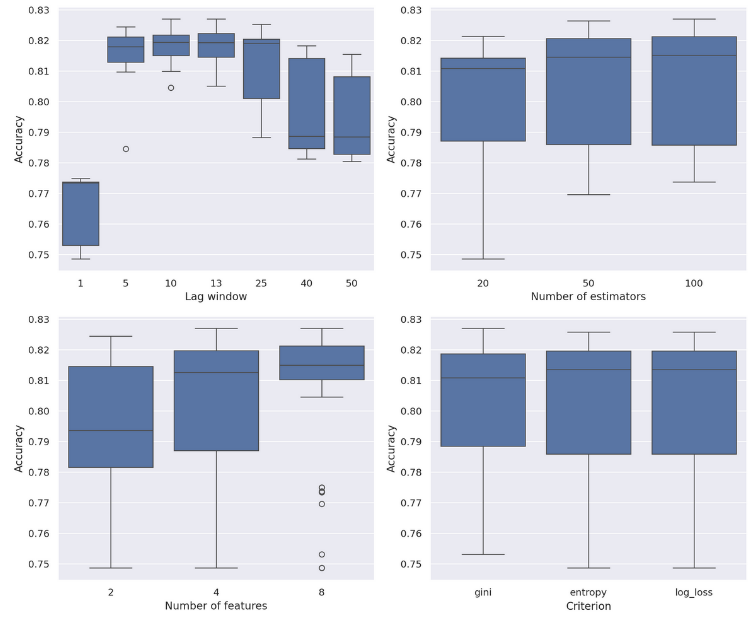
\includegraphics[width=\linewidth]{"pictures/random_forest_results.png"}
	\caption{Results of random forest experiment.}
	\label{fig:random_forest_fig}
\end{figure}















\section{Logistic regression}

Logistic regression is a statistical model used for binary classification.
It calculates the probability of whether a datapoint classifies to one class.
During training of the model a sigmoid function of features of data is calculated that best fits the provided training dataset.

More precisely, the model calculates the function \(Y(X) = \frac{1}{1+e^{-z}}\), where
\begin{itemize}
	\item \(z = B_0 + B_1\cdot X_1 + \ldots + B_n\cdot X_n\),
	\item \(X_1, \ldots, X_n\) are features of data \(X\),
	\item \(B_0, B_1, \ldots, B_n\) are parameters of the model.
\end{itemize}
Function \(Y\) assumes values only in the range \((0,1)\).
If \(Y(X) >= 0.5\), the model classifies the datapoint as 1 (in our model below - the price will be higher). If the converse is true, the datapoint is classified as 0 (the price will be lower).

During training the parameters \(B_0, B_1, \ldots, B_n\) are chosen using Maximum Likelihood Estimation function, so that the results of the \(Y\) function best fit the training dataset.

Two models have been trained.
The first one is trained to predict if the next price in the dataset wil be higher than the previous one, provided with a sequence of prices spanning over the last \verb|num_lags| days.
The second one does the same but operates on monthly averages instead of single records (for this, the dataset was averaged over subsuquent months).
The first model proved to be more precise with an accuracy of 82\% for an optimal value of k of around 40 (Fig \ref{fig:logv1}). At the same time the second model only scored 75\% (Fig \ref{fig:logv2}).

However, simply predicting whether the price will be higher or lower is much easier then predicting the actual next price.
Additionally, logistic regression assumes an independence of datapoints from each other, wherefore it performs poorly for time series datasets.
Therefore this model is insufficient for our purpose.

\begin{figure}[h!]
	\centering
	\begin{subfigure}[b]{0.4\linewidth}
		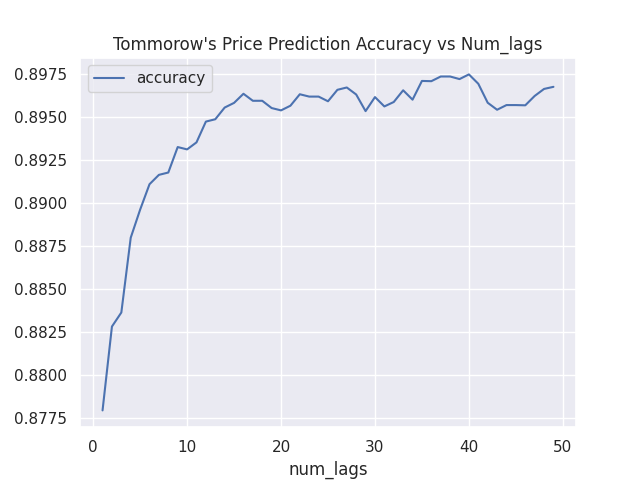
\includegraphics[width=\linewidth]{pictures/logistic-regression-v1.png}
		\caption{Day-by-day prediction.}
		\label{fig:logv1}
	\end{subfigure}
	\begin{subfigure}[b]{0.4\linewidth}
		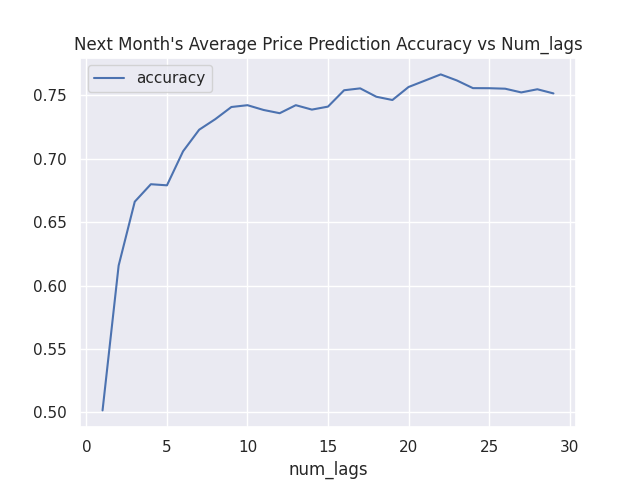
\includegraphics[width=\linewidth]{pictures/logistic-regression-v2.png}
		\caption{Month-by-month prediction.}
		\label{fig:logv2}
	\end{subfigure}
	\caption{Plots of two models of logistic regression.}
	\label{fig:logistic-regression}
\end{figure}












\section{Support vector machine}
Support vector machines are a widely popular model for machine learning classification problems, due to their high generalization abilities and applicability to high-dimensional data.

The model construes datapoints as high-dimensional vectors and finds the best hyperplane that divides the two classes the data is classified into. The goal of training is to find the hyperplane with the greatest margin - that is, the greatest distance from the closest vectors, called the support vectors.

The model uses a kernel function to transform the space of data points which are not separable by a hyperplane, into one where they are separable.

The \(C\) value specifies how accurate the model should be, that is how much it should avoid misclassifications, versus how wide the margins should be. A lower value of \(C\) corresponds to wider margins.

The gamma value specifies how much influence individual training datapoints should have. The \verb|scale| value of gamma means that gamma is scaled automatically to fit the size of the dataset.

% A model was trained to predict whether the next price will be higher or lower than the previous one.

% What was used is Support Vector Regression, which is a modification of the idea of Support Vector Machine for the purposes of regression tasks, where instead of finding a hyperplane, 

The model was tested using two metrics: Mean Squared Error and R-squared.

For the support vector machine there were overall nine models tried:

\begin{itemize}
	\item three kernels: \verb|rbf|, \verb|poly|, \verb|sigmoid|
	\item one gamma: \verb|scale|
	\item three C values: 0.1, 1.0, 10.0
\end{itemize}
The `poly` kernel worked much better than both `rbf` and `sigmoid`, which both worked equally badly. Overall, though, the statistics for every model were terrible. The value of `C` has had very little impact and only on `rbf` kernel.

Support Vector Machine model doesn't perform well in this task, as can be seen in the results (Fig \ref{fig:svm}). Overall, Support Vector Machins don't perform well with large datasets, which will be part of our endeavour.

\begin{figure}[h!]
	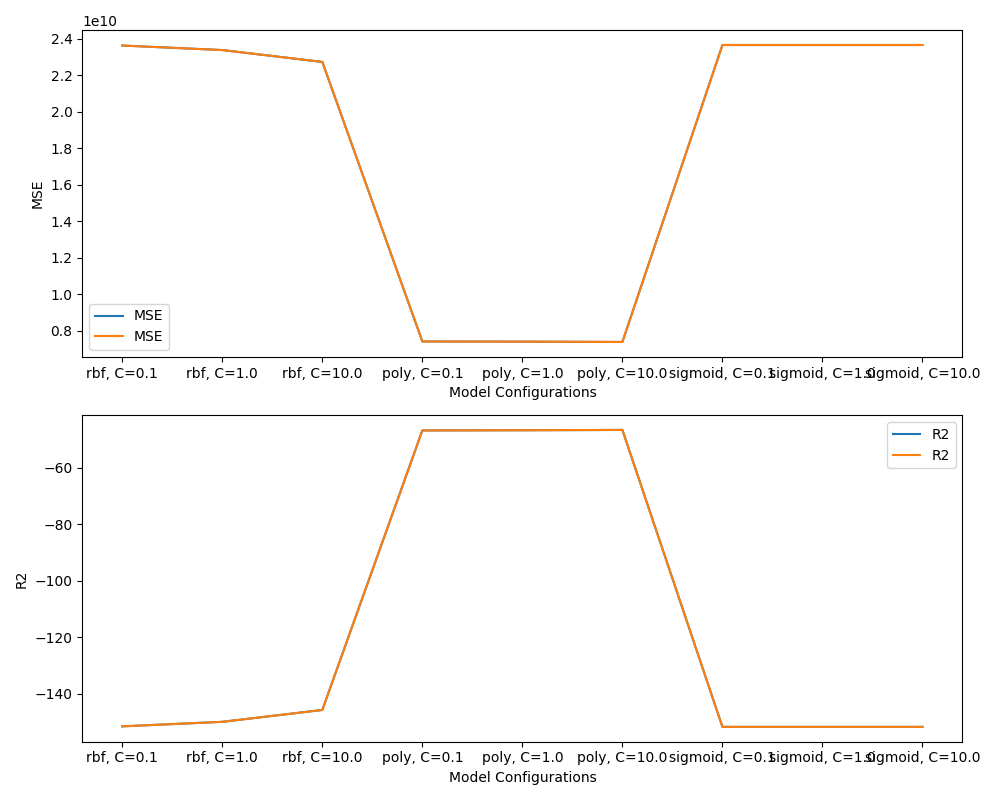
\includegraphics[width=\linewidth]{"pictures/svm_models_results.png"}
	\caption{Results of support vector machine experiment.}
	\label{fig:svm}

\end{figure}
\section{Multi-layer perceptron}
\section{Convolutional neural network}
\section{Residual neural network}
